\section{Theory}\label{Theory}
%%%%%%%%%%%%%%%%%%%%%%%%%%%%%%%%%%%%%%%%%%%
\subsection{Gyrotron guns and trapping phenomena}\label{Section_gyrotron}


Gyrotrons are microwaves generator devices used in plasma heating and current drive applications for fusion purposes \cite{Pagonakis}. The operating mode of gyrotron guns is based on the electron cyclotron maser instability (CMI). This instability occurs when a beam of relativistic electrons, gyrating around magnetic field lines, interact with the transverse component of the electric field. The transverse electrons' energy is then converted in electromagnetic waves in an open, resonant cavity. More precisely, the interaction takes place between the electron beam and a transverse electric mode TE$_{m,p,q}$ supported by the cavity, see Fig.(\ref{modes}) - Left. The subscripts $m,p,q$ denote respectively the azimuthal, radial and longitudinal mode numbers. When the pulsation of the EM wave inside the cavity equals the relativistic electron cyclotron (EC) frequency, that is $\omega = \omega_e/\gamma$, a group of electrons with initially no phase relation, will, under the action of the field, regroup and gyrate in phase, as a whole. This is called 'phase bunching', see Fig.(\ref{modes}) - Right. Note that we define $\omega$, $\omega_e$ as the EM wave and the EC frequencies respectively, and $\gamma$ the Lorenz factor.  Then, increasing the frequency $\omega$, after an integer number of periods, the electrons will be in a region such that their transverse velocity is on average positive, $\braket{v_x} > 0$ \cite{AlbertiThesis}. Using that the electrons energy $W$ varies as $dW/dt = -|e|v_xE_x$, the energy variation is negative, and by conservation, the latter is converted in EM energy.\\

\begin{figure}[h!]
\centering
	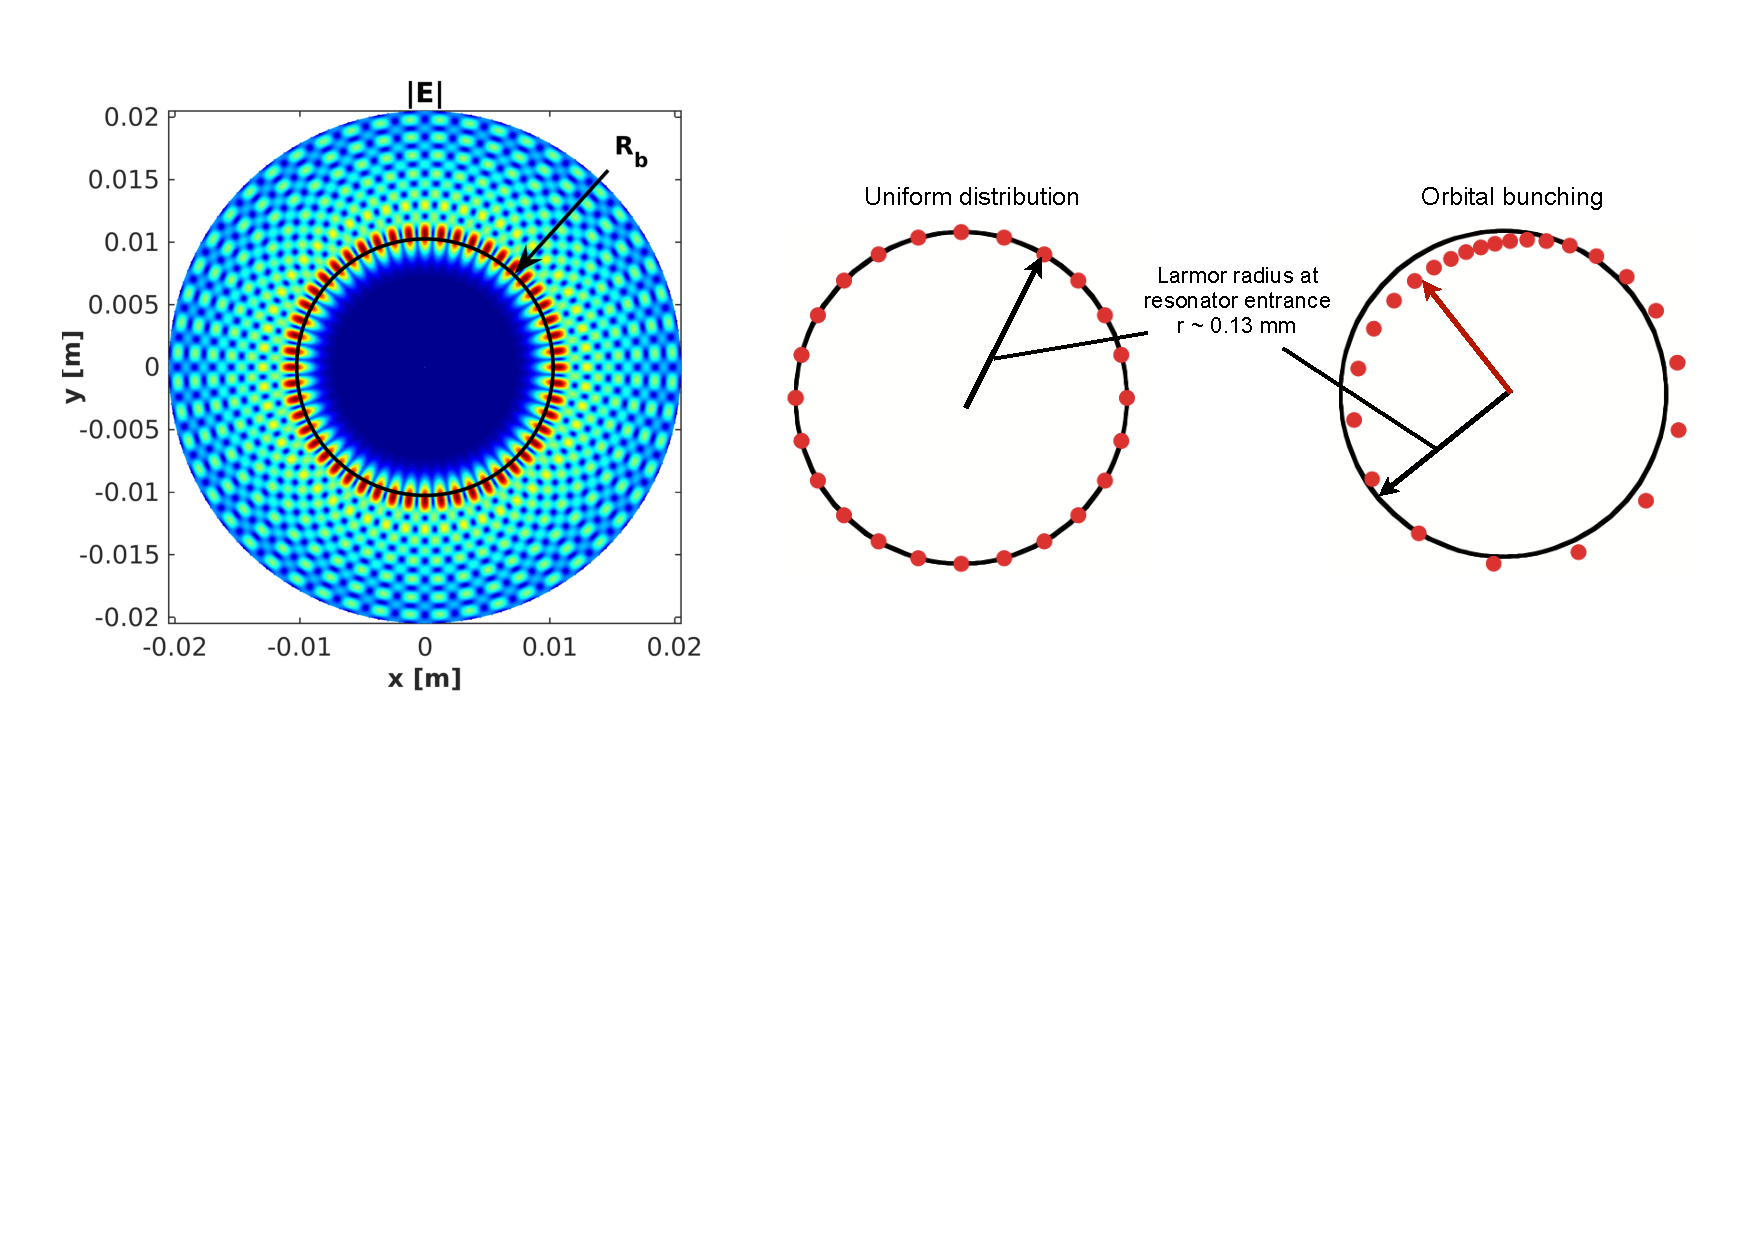
\includegraphics[width = 1 \textwidth]{gyrotron_TE_bunching}
	\caption{\label{modes}Left: Amplitude of the electric field profile in the transverse cross-section for the mode TE$_{26,7}$ of Tokamak à Configuration Variable (TCV) dual-frequency gyrotron  \cite{GenoudThesis}. The black circle represents the annular electron beam. - Right:  Orbital bunching mechanism of electrons in the cavity (resonator). Electrons are shown by red dots, and the black circle corresponds to a Larmor orbit. Source: courtesy of S. Alberti.}
\end{figure}  

\begin{figure}[h!]
\centering
	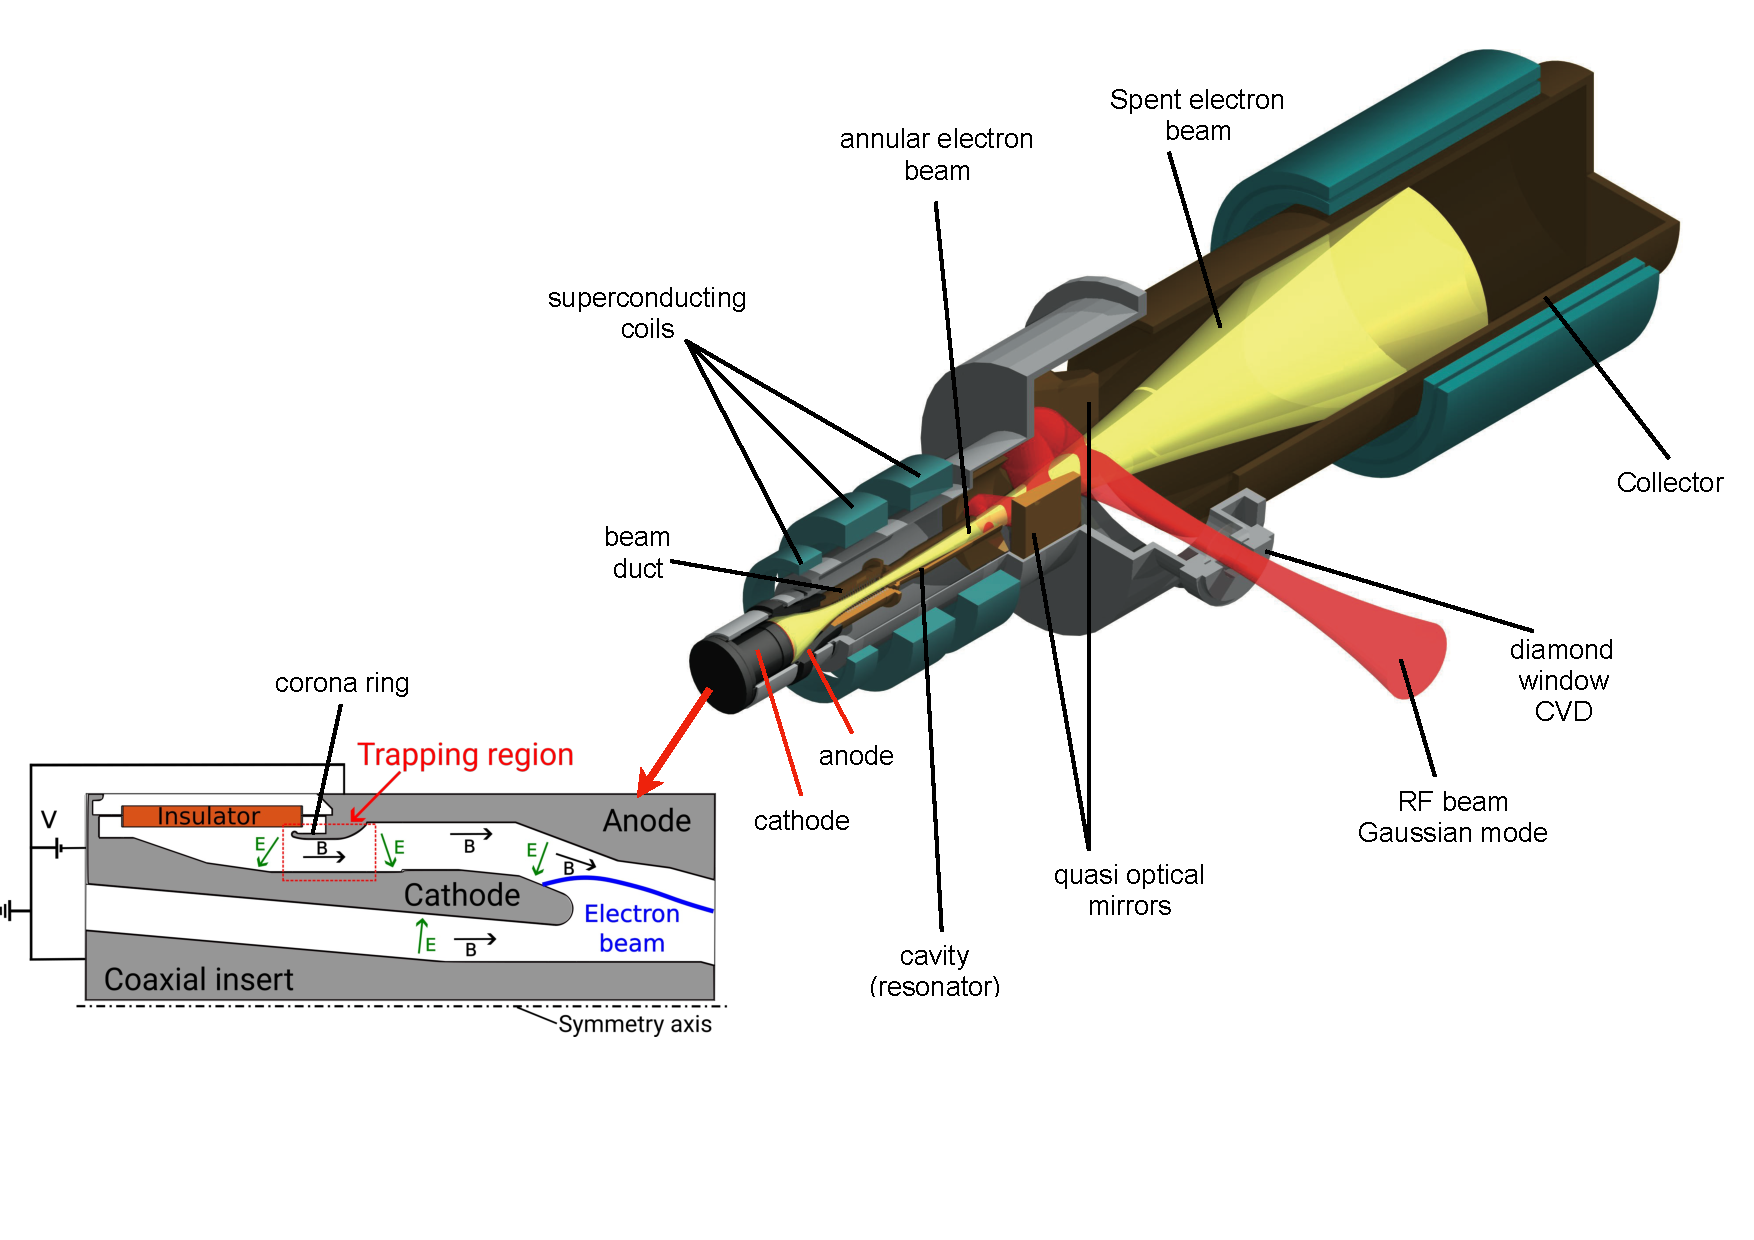
\includegraphics[width = 0.85 \textwidth]{gyrotron_schematics_3}
	\caption{\label{gyrotron} Right: Schematic of a gyrotron gun and its different constituents. Source: courtesy of S. Alberti - Left: Zoomed view of the MIG from the gyrotron \cite{TREX}.}
\end{figure}  

\noindent On top of the cavity lies a mode converter so that the frequency of the emitted microwaves matches one of the plasma resonance frequencies. The radiation is then reflected by several mirrors and directed through a diamond window so it can penetrate the plasma, see Fig.(\ref{gyrotron}). The most common heating frequency corresponds to the electrons' gyrofrequency $\omega_e$, or some of its harmonics. In that case, we speak of electron cyclotron resonance heating (ECRH). It is when the electromagnetic wave has a component along the toroidal magnetic field that it can induce a current. The latter phenomenon is called electron cyclotron current drive (ECCD).\\

All the previously described events occur in the gyrotron cavity, or after the latter. However, the beam quality as it enters the cavity is very important, since it will, among others, participate to the interaction efficiency \cite{Pagonakis}. The beam is generated by an electron gun, also called magnetron injection gun (MIG). An axial cross section of the MIG is depicted in the left part of Fig.(\ref{gyrotron}). It consists in a cylindrical cathode around a coaxial insert, and a cylindrical anode of a larger radius around it. The beam electrons are produced by thermo-emission. The electrons are accelerated by the electric field and guided through the exit of the MIG by mean of the magnetic field present as shown in Fig.(\ref{gyrotron}), so they can reach the cavity where they will achieve the collective gyro-motion from the CMI. Nevertheless, multiple phenomena can disrupt the functioning of the MIG, among which the formation of trapped electron clouds in the rear part of it \cite{Pagonakis, lebars_et_al}. Indeed, as the local population of electrons increase inside the MIG cavity, discharges phenomena can occur when a certain critical value is reached. Thus, voltage stand-off problems can follow from discharges \cite{ITER_gyrotron}, that were later attributed to the presence of these trapped electrons. Regarding the trapping in itself, electrons can accumulate in a cloud for several reasons, as among others, the so-called adiabatic trap, or the potential well trap. In this report, we will focus on the second. Let us first briefly summarise this type of trapping mechanism.\\

\begin{figure}[h!]
\centering
	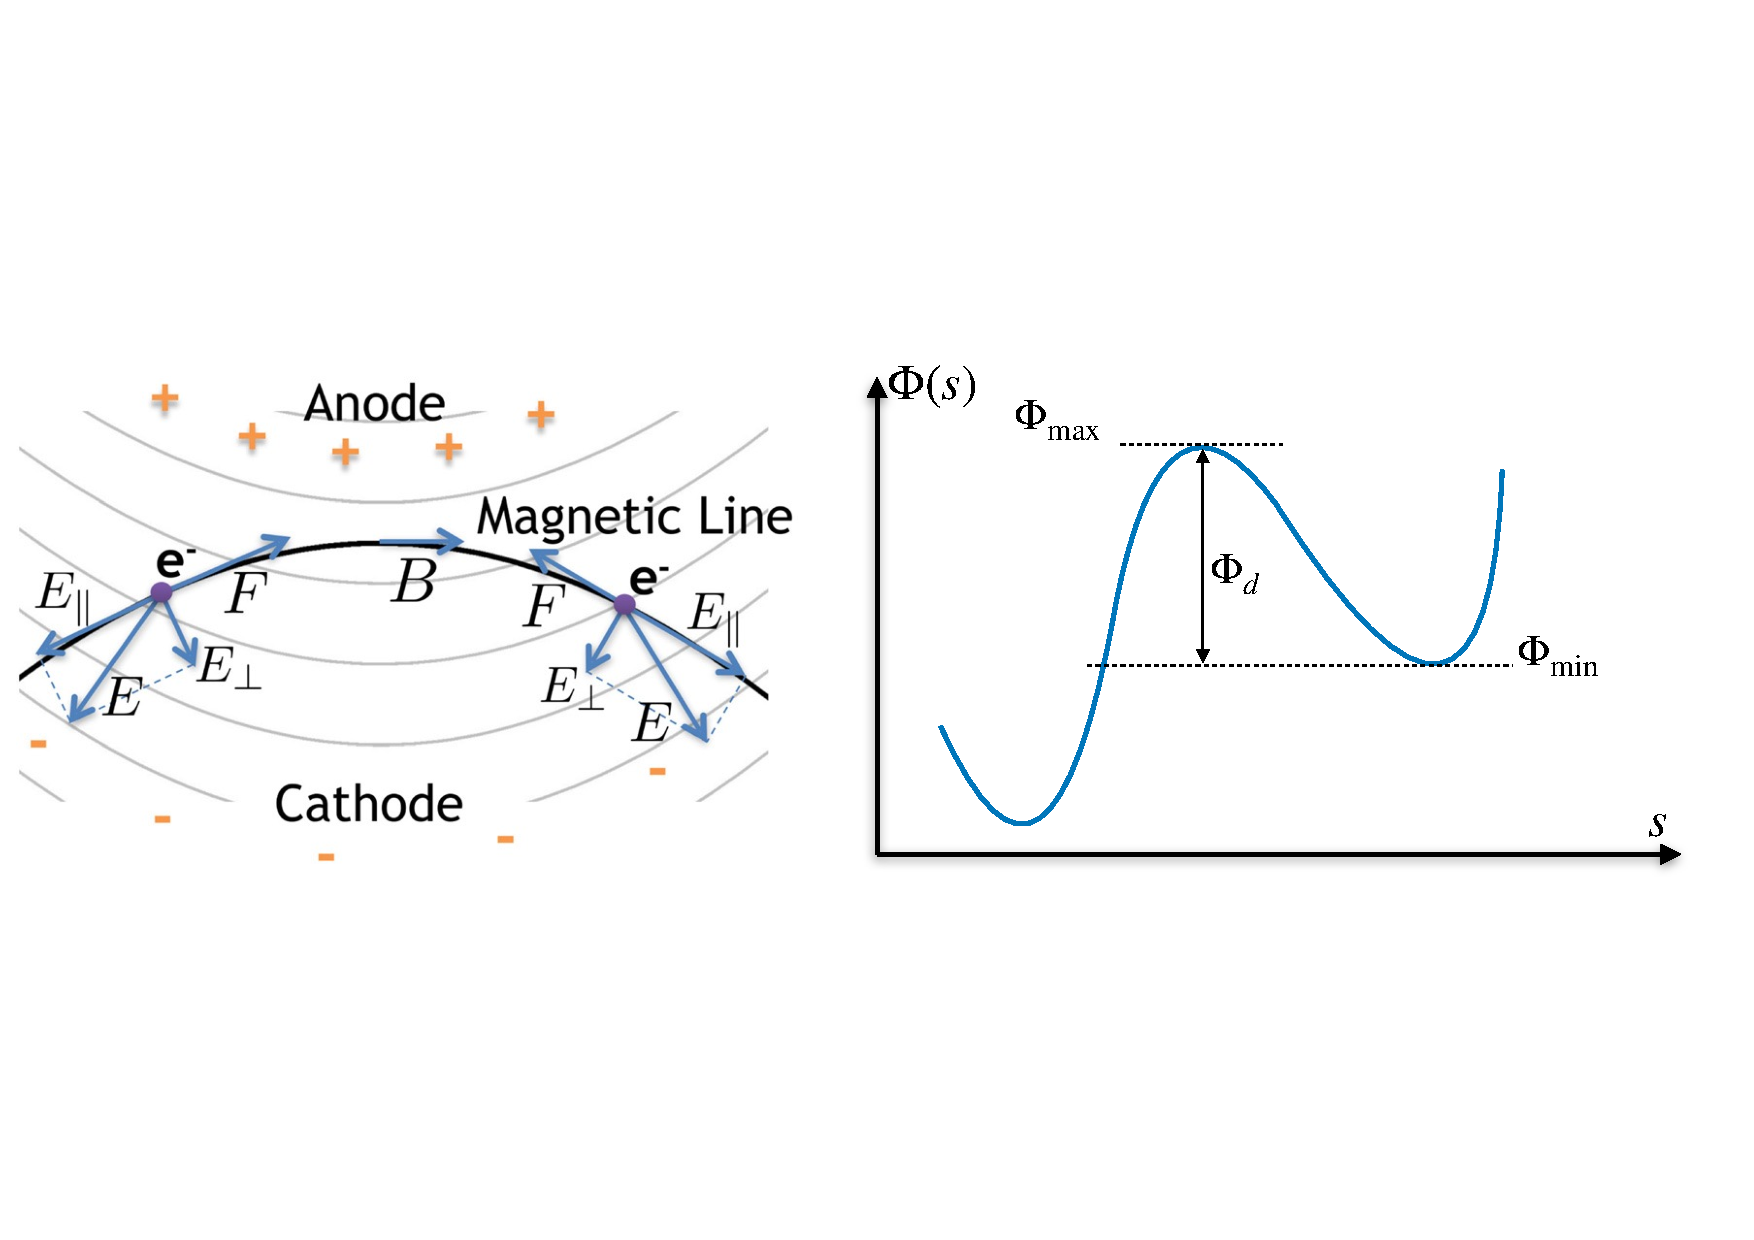
\includegraphics[width = 1 \textwidth]{potential_well}
	\caption{\label{mag_well} Left: configuration favorable to the formation of a potential well. The equipotentials are depicted by plain, grey lines, while the magnetic field line is represented by the black one \cite{Pagonakis} - Right: Potential-well definition. The curvilinear abscissa along the field line is denoted by $s$.}
\end{figure} 


A magnetic potential well can form every time a magnetic line intersects twice an equipotential as depicted in Fig.(\ref{mag_well}). Indeed, in such a configuration, the electrons are accelerated on one side of the well and decelerated on the other side by the Coulomb force projected along the field line $F_{\|} = -eE_{\|}$. The potential well is characterised by its location as well as its depth, which is defined locally as the difference between the local maximum $\Phi_{max}$ and the highest of the local minima on both side of $\Phi_{max}$. Hence, the depth reads $\Phi_d = \Phi_{max} - \max{\{\Phi_{min}\}}$. Thus, the electrons oscillate inside that well around its center, while the component $E_{\perp}$ of the electric field contributes to an azimuthal drift $\mathbf{v_d} \propto \mathbf{E}_{\perp} \times \mathbf{B}$, causing the electrons to gyrate around the MIG symmetry axis, giving the cloud an annular shape.\\

%%%%%%%%%%%%%%%%%%%%%%%%%%%%%%%%%%%%%%%%%%%%%%%%%%%%%%%%
\subsection{TRapped Electrons eXperiment TREX}\label{TREX_Section}

In order to emphasize experimentally the mechanism of electron trapping by magnetic potential well as described in \ref{Section_gyrotron}, an experiment is, at the time of writing, being built at the Swiss Plasma Center (SPC) \cite{TREX}. The TREX experiment aims at studying the formation of electron clouds under multiple gyrotron's magnetic, electric and neutral pressure configurations. One sees indeed that the outer electrode designed as shown in Fig.(\ref{TREX_schematics}) is an approximate replica of the corona-ring from MIG. 

\begin{figure}[h!]
\centering
	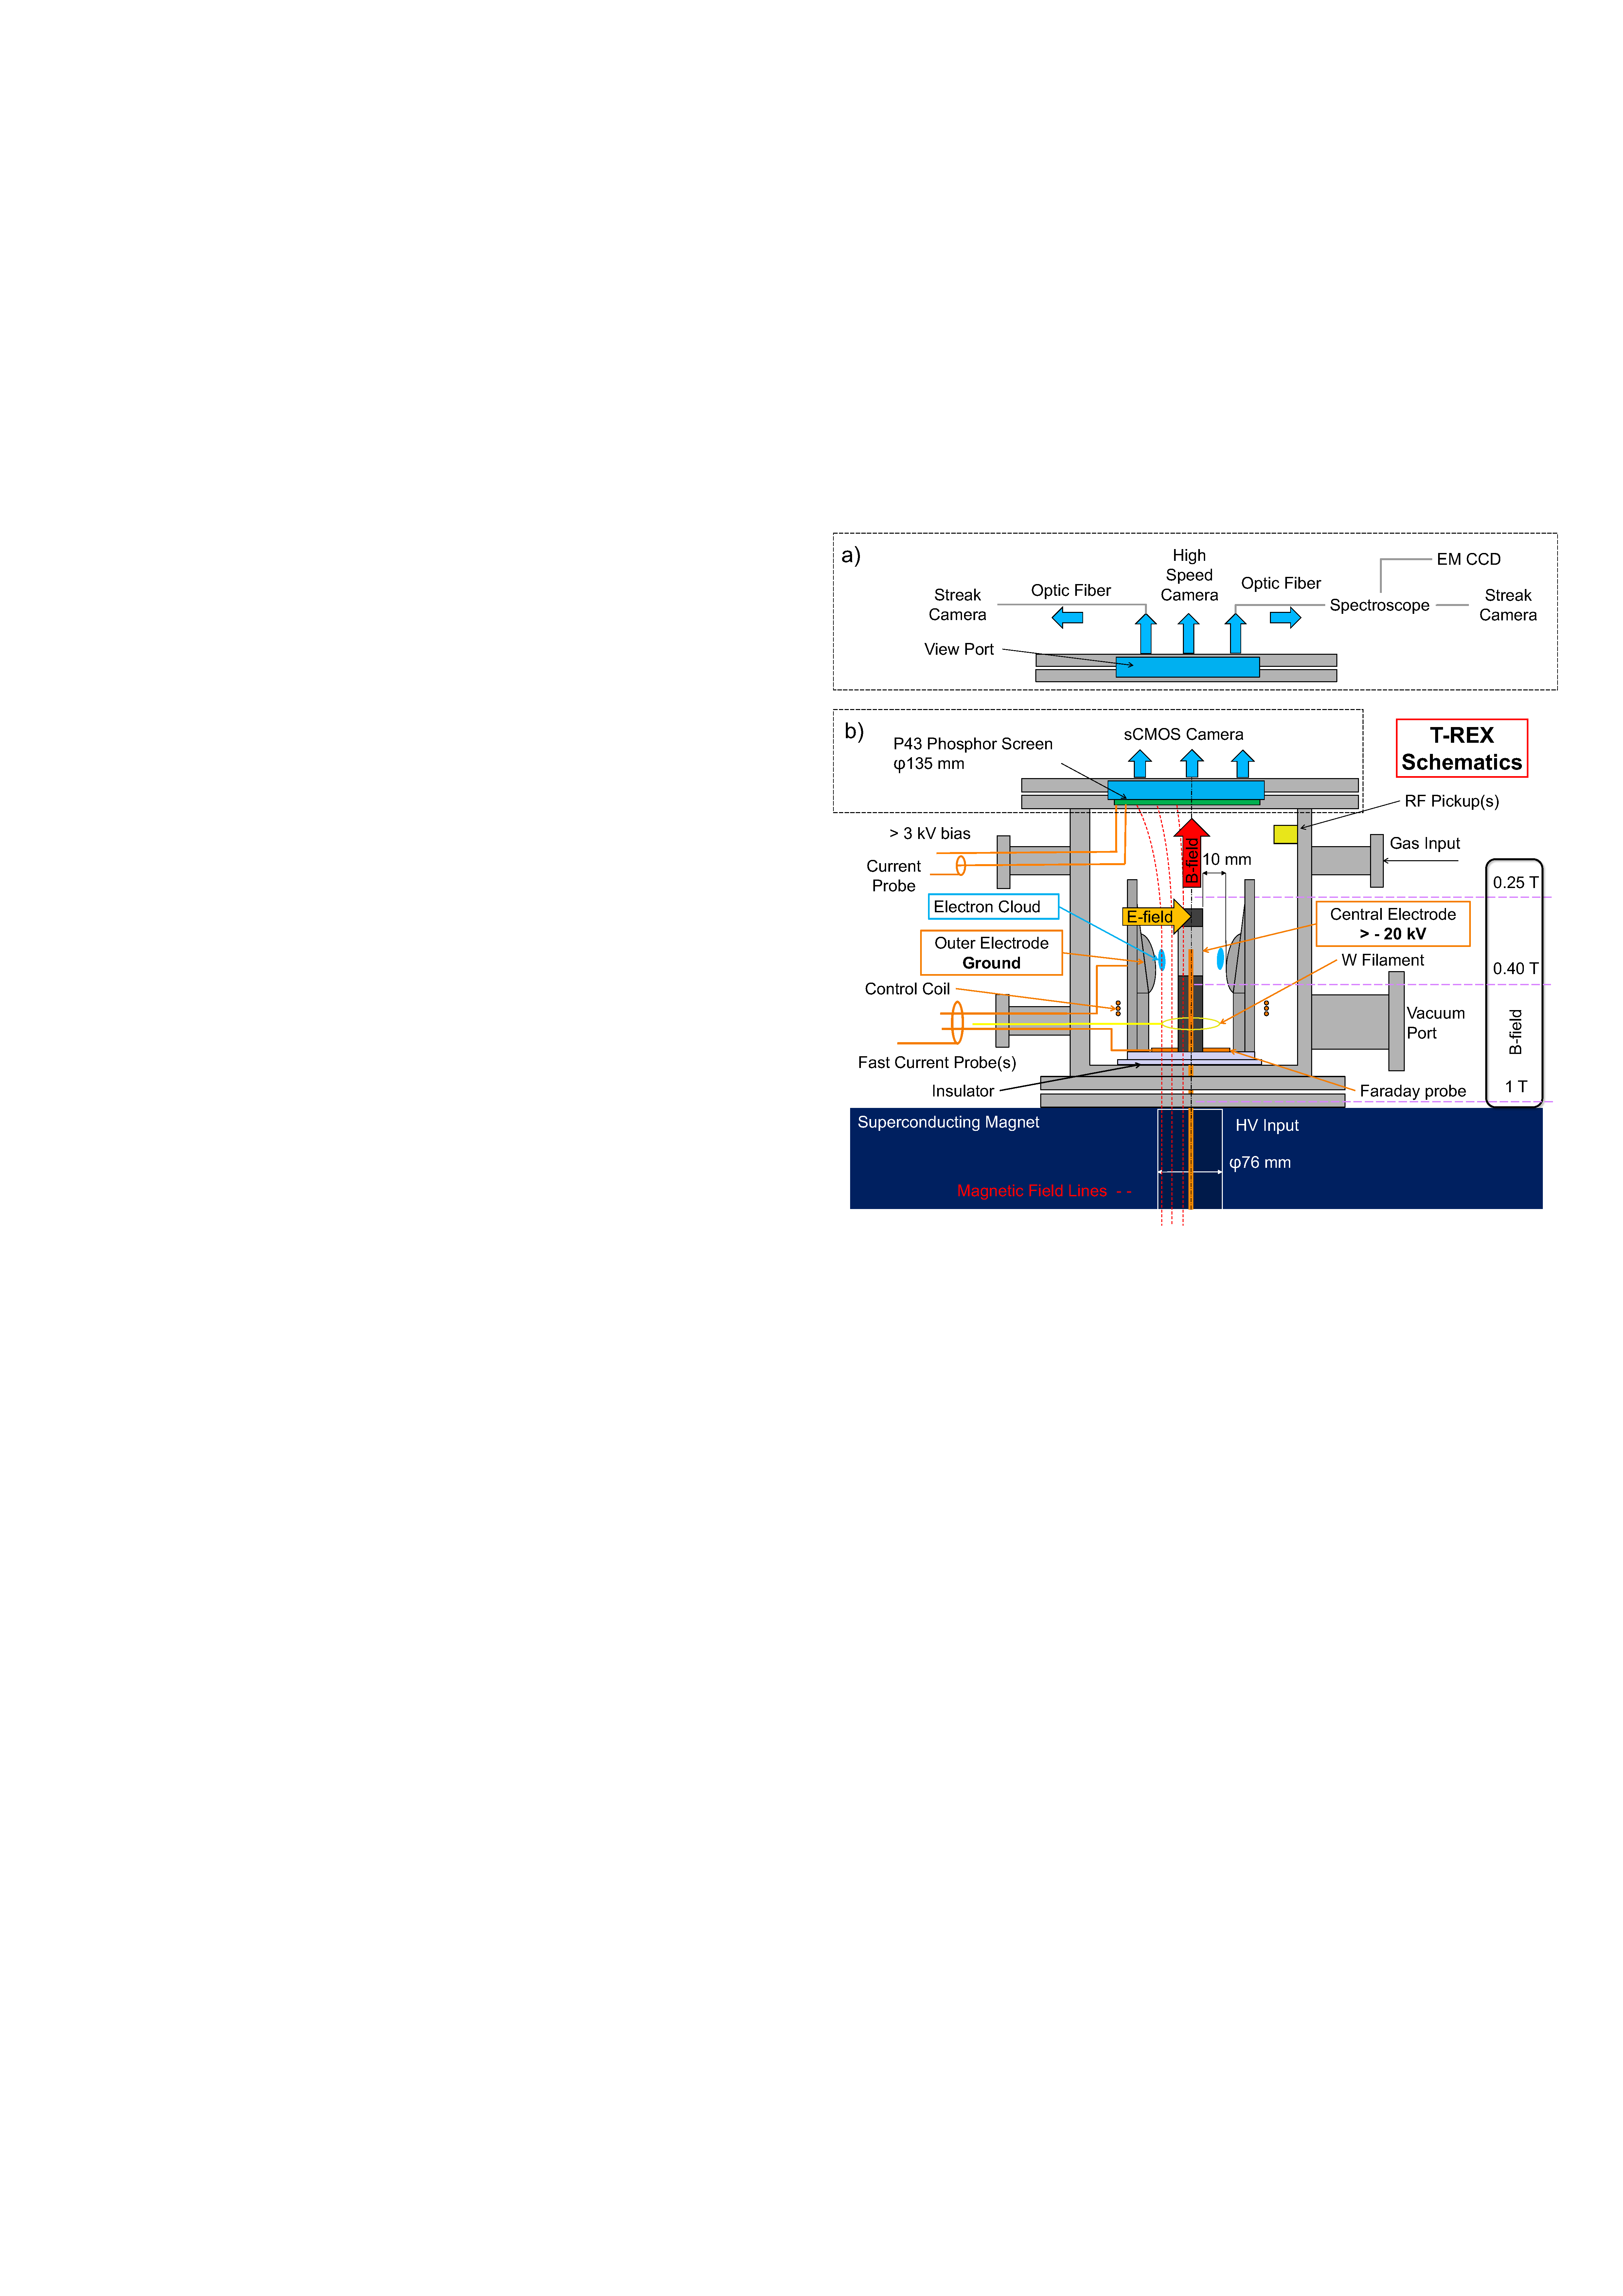
\includegraphics[width = 0.65 \textwidth]{TREX_schematics}
	\caption{\label{TREX_schematics} Schematic of the TREX experiment \cite{TREX}.}
\end{figure}  

Regarding the experiment design in itself, the chamber is set on top of a superconducting magnet, such that the magnetic field lines run through the chamber axially. The potential bias between the two electrodes is planned to be of about $\Delta \Phi=20$ kV and the electric field topology is changed locally by mean of amovible and interchangeable electrodes. The magnetic field intensity is kept between  $0.25 - 1.0$ T, and the neutral pressure should range as $p=10^{-7}$ to $10^{-5}$ mbar. A tungsten filament can act as a source of electrons, although it has been shown by \cite{lebars_et_al} that background radiation could be sufficient in certain geometries, to provoque the formation of a cloud. The optical diagnostic methods consist in either a sCMOS camera on top of a biased phosphor screen, or streak camera working together with a high speed camera as well as a spectroscope. When neutralising the cloud by switching off the high-voltage source, the cloud would follow the field line and be directed towards the phosphor screen, enabling to measure the current through it, and the image would be taken by the sCMOS camera. The experiment being built currently, the design is guided by some FENNECS code results, and some numerical characteristics as the expected cloud density were deduced from simulations too. The experimental results are to be confronted to the code ones. \\


%%%%%%%%%%%%%%%%%%%%%%%%%%%%%%%%%%%%%%%%%%%%%%%%%%%%%%%%%
\subsection{The FENNECS code}\label{fennecs_section}
In order to model the electron trapping in various geometrical situations, the FENNECS code \cite{fennecs} was used. It is a 2D3V particle-in-cell code, that solves the Poisson-Vlasov system from Eq.(\ref{PoissVlas}) in cylindrical geometry, for the distribution function $f_e$ and the electrostatic potential $\phi$. It has been developed in order to show the self-consistent formation of electron-clouds in gyrotron guns, due to the ionisation of the residual neutral gas (RNG) present in the gyrotron cavity \cite{lebars_et_al}.  

\beq
\begin{split}
&\Big(\frac{\dd}{\dd t} + \mathbf{v}\cdot \frac{\dd}{\dd\mathbf{x}} + \frac{e}{m_e}\left(\mathbf{E} + \mathbf{v}\times \mathbf{B}\right) \cdot \frac{\dd}{\dd \mathbf{v}}\Big) f_e(\mathbf{x}, \mathbf{v}, t)=0,\\
&\nabla^2 \Phi(\mathbf{x},t)=-\frac{e}{\epsilon_0}\int f_e(\mathbf{x}, \mathbf{v}, t)d^3\mathbf{v}.
\end{split}\label{PoissVlas}
\eeq  

\noindent FENNECS is a highly parallelised code in the sense that it uses both multiple nodes (MPI) and multiple core per node (openMP). Regarding numerical methods, the code uses cylindrical coordinates, and axisymmetry is assumed, so that $\dd \theta = 0$, $\theta$ being the poloidal coordinate. The poisson equation is solved using finite elements, based on weighted extended b-splines, whereas the collisional Vlasov equation is solved by sampling the electron distribution $f_e$ with macro-particles, then calculating the trajectory of each macro-particle by mean of the Boris algorithm \cite{lebars_et_al, BorisAlg}. So far, the code only takes account for primary ionisations coming from electron-neutral collisions, where electrons collide with the RNG. In fact, the ions having a Larmor radius of the order of the meter, they are collected at the cathode, during times much shorter than the average ionisation time. Indeed, being generated with approximately zero velocity (the RNG atoms have zero velocity in the code), the ions characteristic 'living' time is roughly $\tau_l \sim \Delta r/ v_{\mathbf{E}\times \mathbf{B}}$, $\Delta r$ being of the order of the distance between the electrodes ($\sim$cm), which is much shorter that the ionisation time. Taking $B\sim0.2$ T, $\Delta\Phi \sim 2\cdot 10^4$ V and $\Delta r \sim 10^{-2}$ m, with $\Delta \Phi$ the electrostatic potential bias between the electrodes, one gets that $\tau_i \sim 10^{-9}$ s. Although this estimate is very rough, for a pressure of $10^{-6}$ mbar, characteristic of gyrotron guns, the ratio of the ions living time to the characteristic ionisation time is of about $\tau_l/\tau_{io}\sim 10^{-6}$ \cite{lebars_et_al}. Thus, the ions-neutrals collisions are neglected, and the electrons-neutrals collisions are implemented using a Monte-Carlo method.\\

\noindent However, although ions-neutral collisions are neglected in the ionisation process, the ions contribution in the formation of electron-clouds can be non-negligible, since when they impinge on the cathode, some electrons can be generated at the metallic surface, by various emission phenomena \cite{baragiola}. The ion-induced electron-emissions will be the object of the following study, having first to be implemented in the code, before to be compared with situations where electron clouds form self-consistently, without taking account for IIEE.
    
%%%%%%%%%%%%%%%%%%%%%%%%%%%%%%%%%%%%%%%%%%
\subsection{Ion-Induced Electron-Emissions}\label{IIEE_section}

In order to take into account IIEE in the FENNECS code, the question of choosing the appropriate physical model arose. Indeed, expected energy distribution of the ions in the TREX experiment was ranging between 0 and 20-30 keV. These values correspond to roughly the minimal and maximal values that could be reached by ions accelerated in an electric field perpendicular to the magnetic field lines, in vacuum, and over a distance of about 1cm. Fig.(\ref{Config_ions}) shows the initial distribution of protons in the coaxial geometry with the $(\mathbf{E}, \mathbf{B})$ configuration described previously, where the electric equipotentials are plotted in blue, and the magnetic field lines in black. In this particular configuration, in vacuum, the acquired energy of the protons when they reach the cathode follows 

\beq
E(r_0) = \Delta \Phi \frac{\log{(\frac{r_0}{r_a})}}{\log{(\frac{r_b}{r_a})}},\label{ions_energy}      
\eeq
 
\noindent where $r_0$ is the initial proton radial position, $\Delta \Phi$ the potential bias between the cathode located at $r_a$ and the anode located at $r_b$. Thus, taking numerical values such as $\Delta \Phi = 20$kV and evaluating $E(r_a)$ and $E(r_b)$, one get that $E\in [0,20]$ keV. This way, a model describing IIEE in this energy range had to be found.\\


\begin{figure}[h!]
\centering
	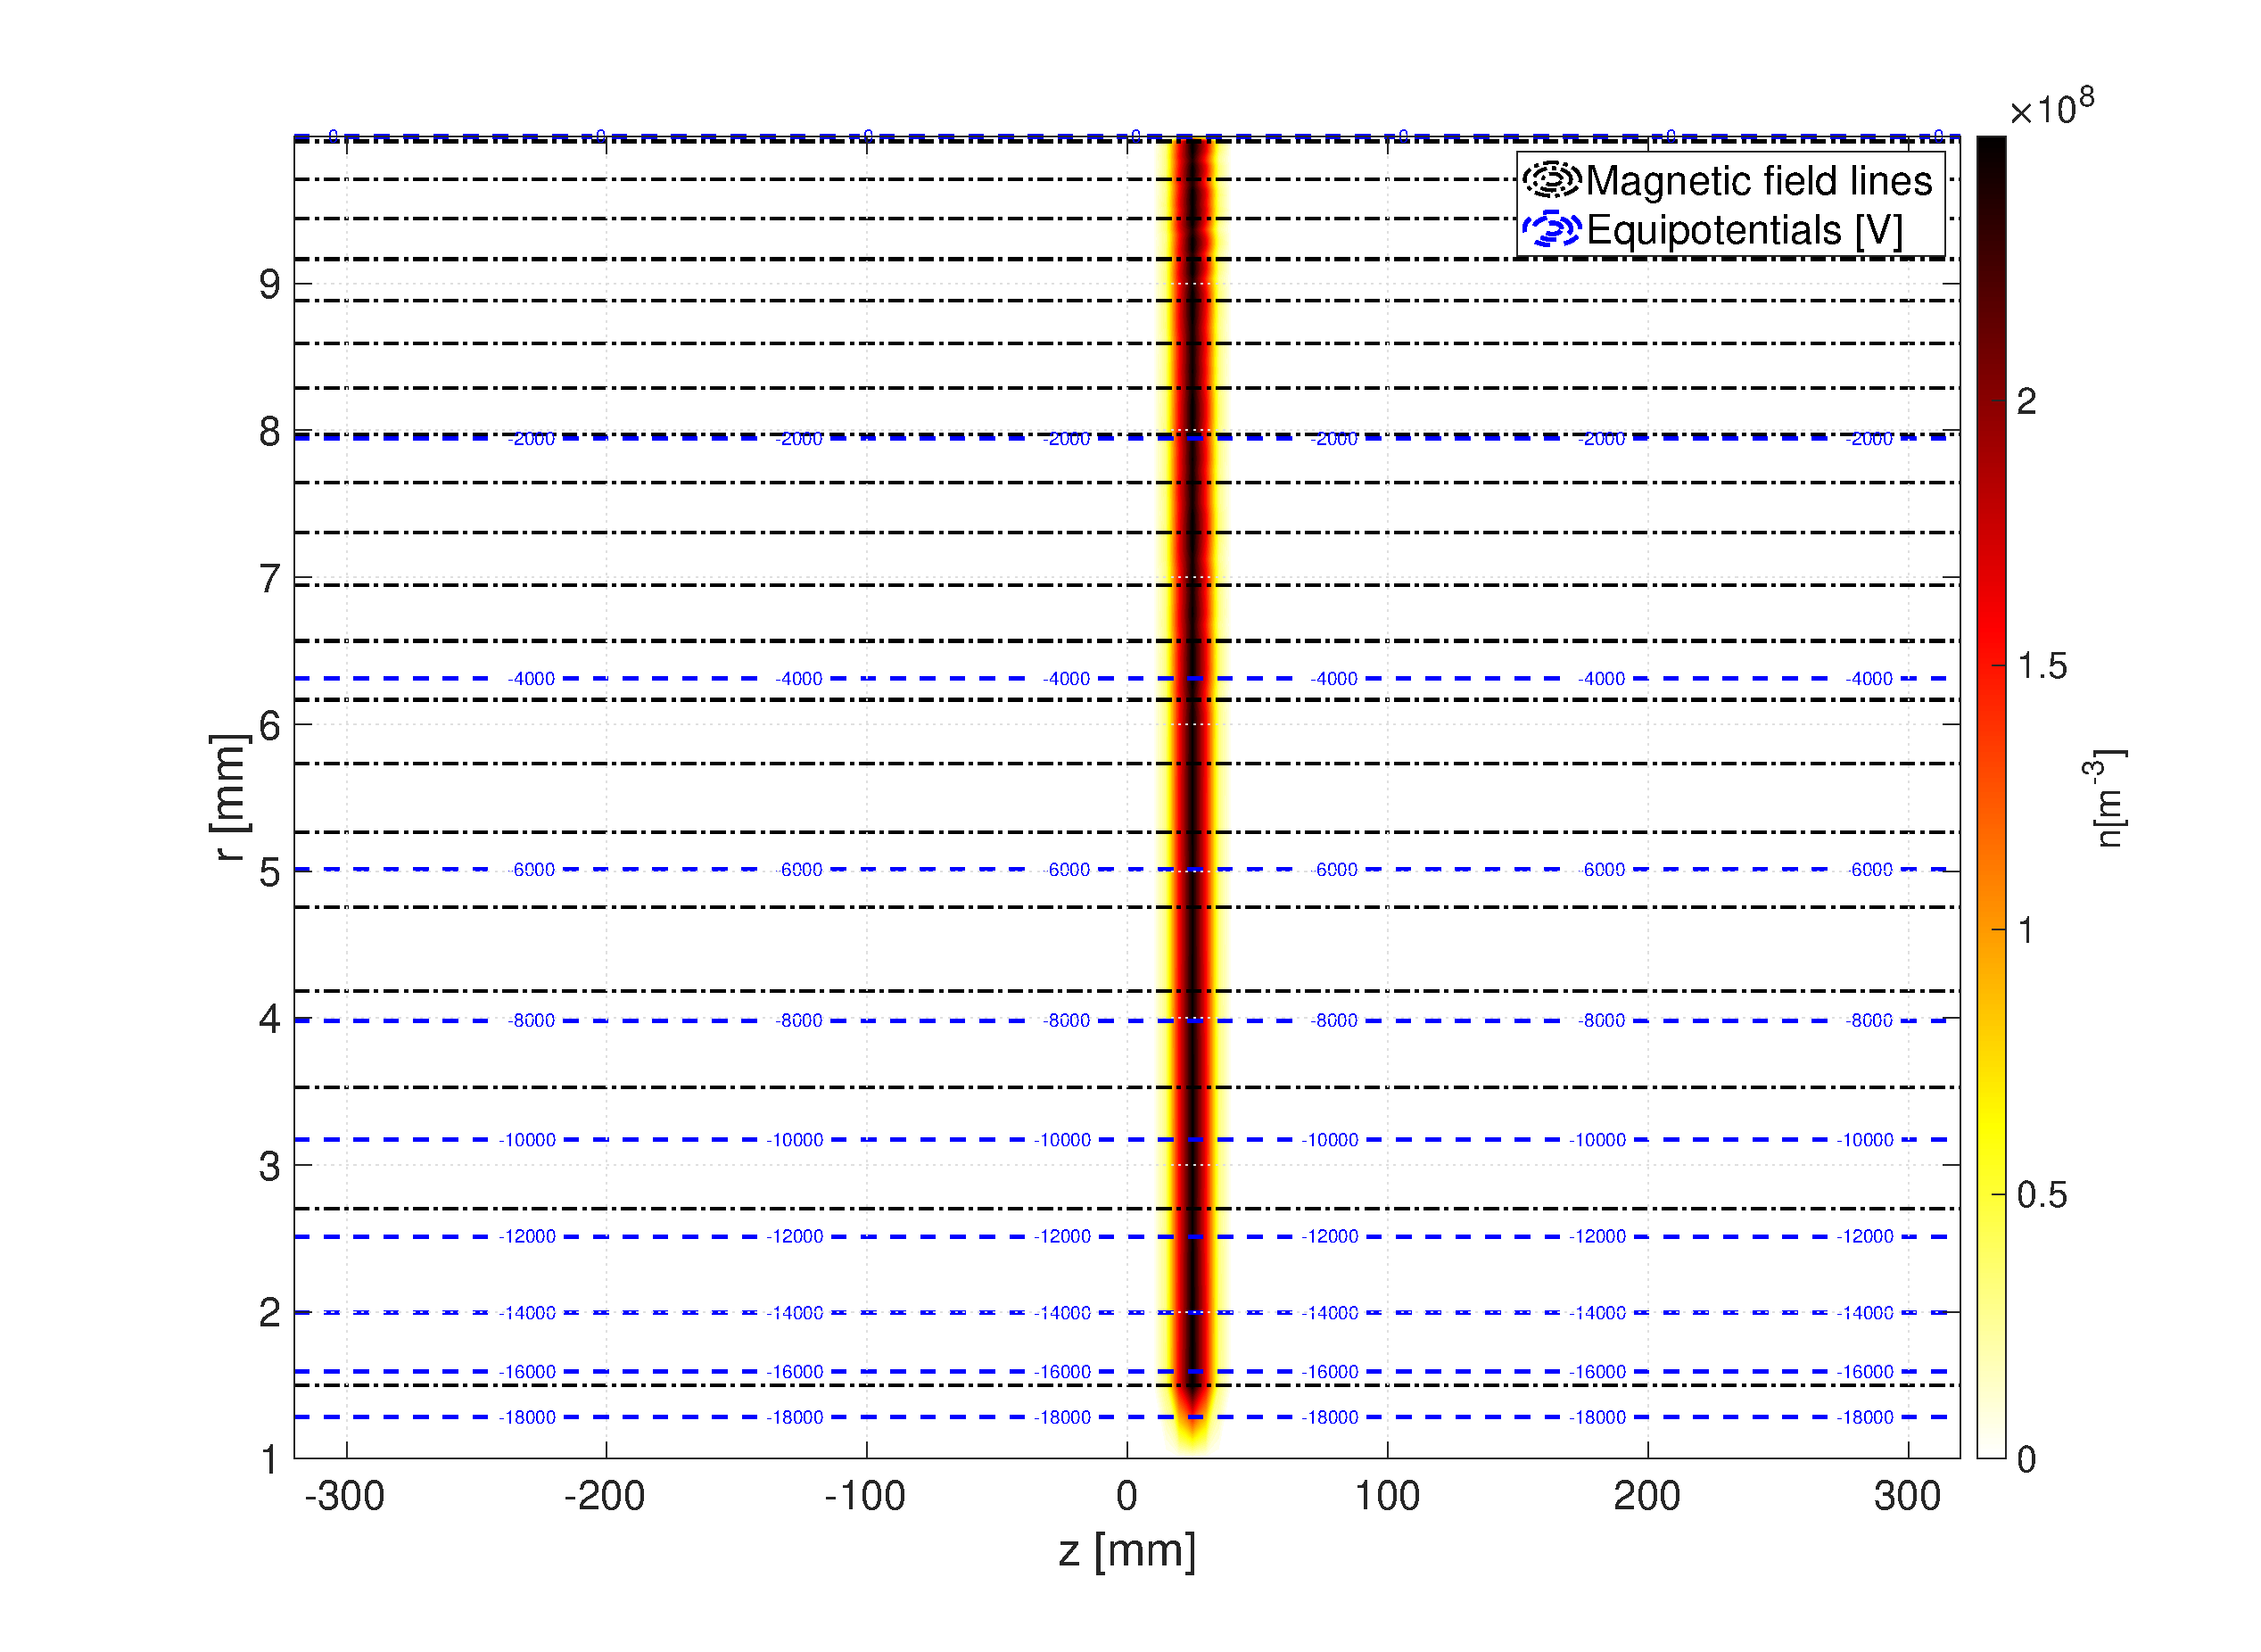
\includegraphics[width = 0.6 \textwidth]{Configuration_ions.eps}
	\caption{\label{Config_ions} Initial ion configuration in ($R,Z$) plane. The geometry is coaxial. Azimuthal symmetry is assumed.}
\end{figure}



\begin{figure}[h!]
\centering
	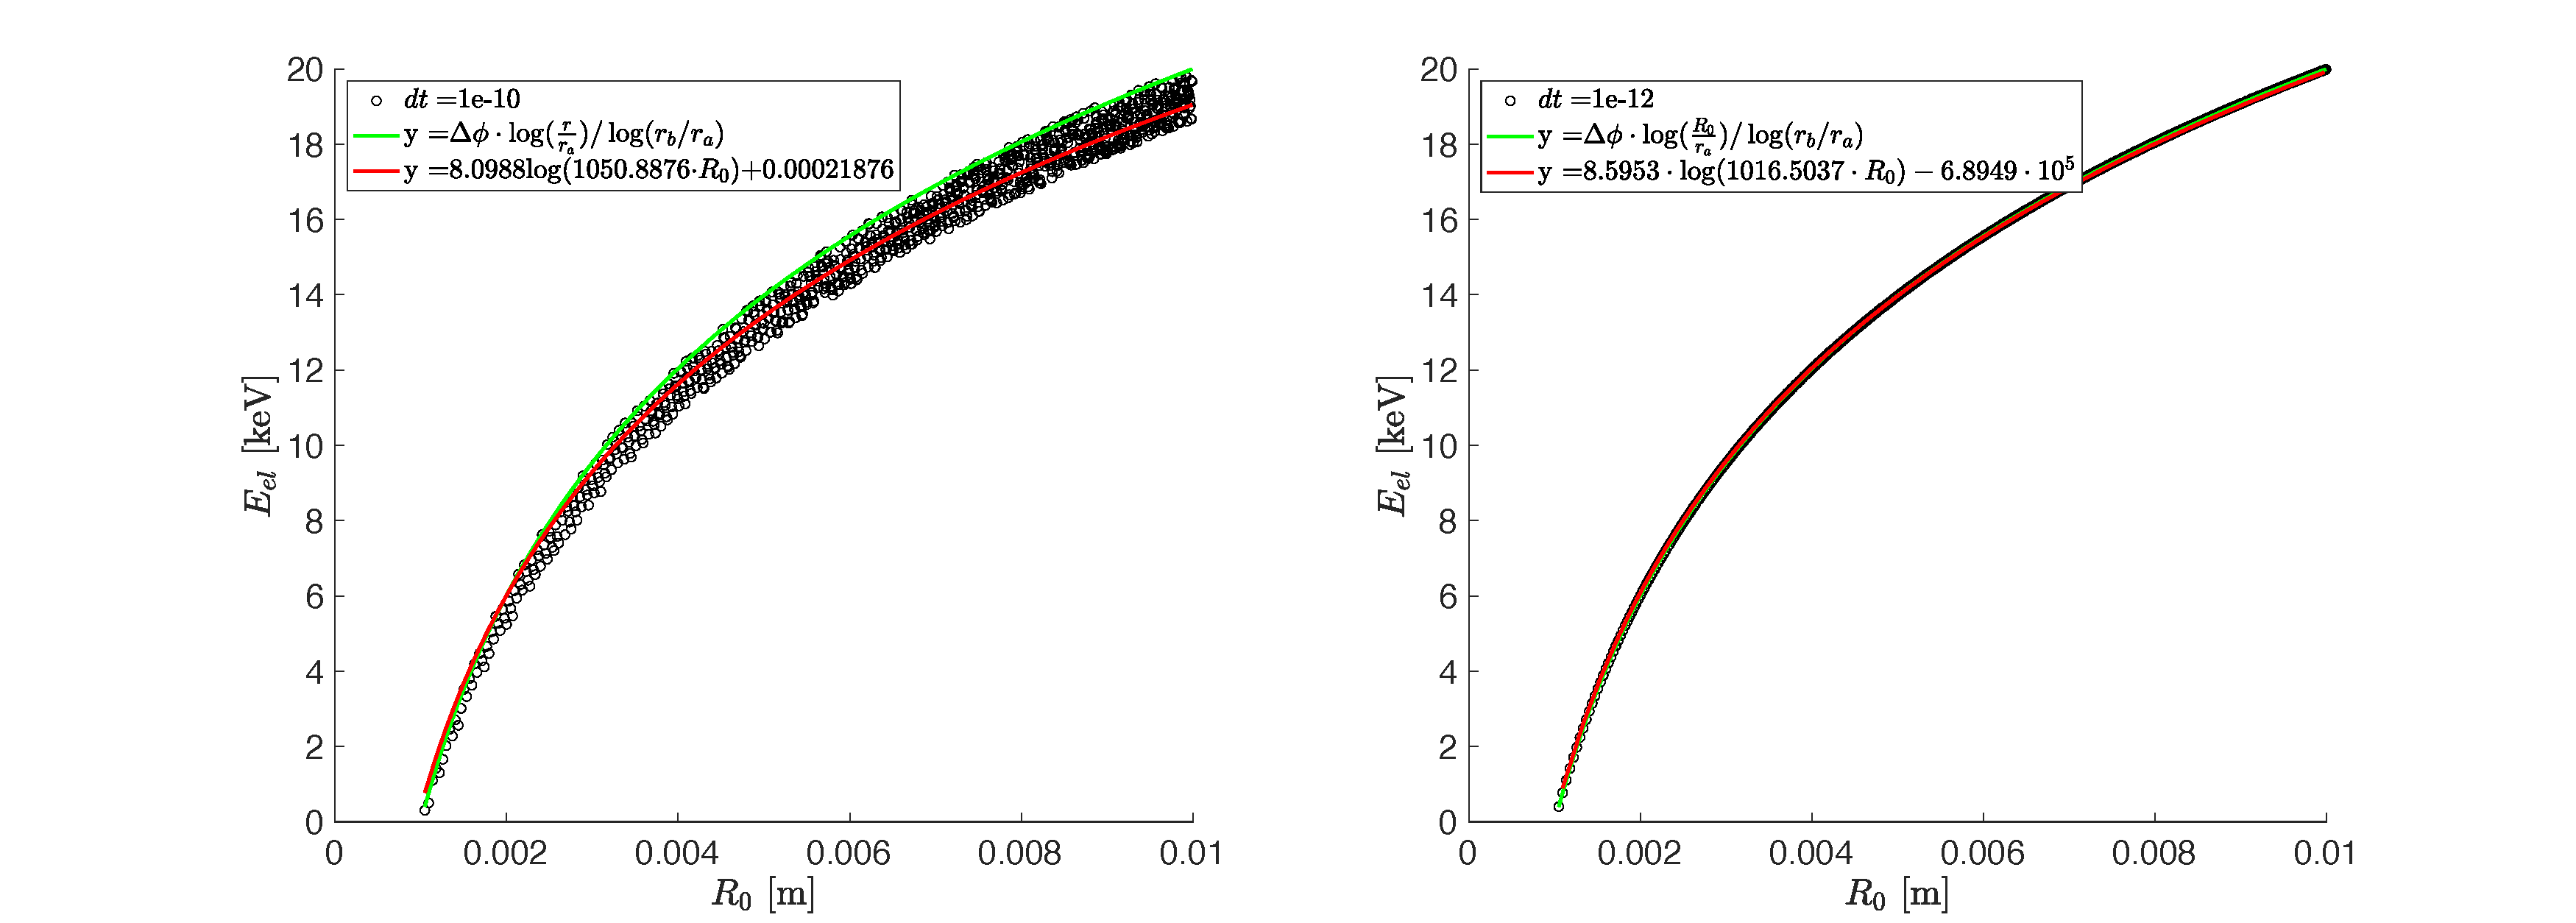
\includegraphics[width = 1 \textwidth]{vert_slice_spread.pdf}
	\caption{\label{vert_spread} Left: energy of the collected ions as they hit the cathode, $dt=10^{-10}$ s. The red curve is the analytical expression for the energy, corresponding to the vacuum electric potential. The red curve is a fit of the data. - Right: Same with $dt=10^{-12}$. }
\end{figure}  



\noindent Regarding the model in itself, one had to consider that IIEE would be dependent on the material constituting the electrodes. Indeed, protons impinging on stainless steel would not have the same effect as if they were striking a copper electrode. The electron yield would also depend on the energy of the incident particle. It was expected that the number of released electrons would be different if the ion hit the cathode at high or low energy. At this point, nothing ensured that the type of interaction between ion an electrode would be the same on the whole energy range. It was also expected that the electron yield would depend on ions parameters: mass $m$, charge $q$ or charge to mass ratio $q/m$ for example. \\

\noindent With these considerations, one model drew our attention: Schou's model, derived by Schou in 1980. Our motivation for a qualitative (at first) survey of these ion-induced electrons drove us towards this model in particular, since it distinguishes itself by its remarkable simplicity. Following the description of Schou's model from \cite{HasselII}, this approach of IIEE is based on the ionisation cascade theory, and a system of Boltzmann transport equations.  Neglecting recoil ionisation in the material, the electron yield $\gamma$ takes the following form: 

\beq
\gamma = \Lambda \cdot D_e,
\eeq

\noindent where $D_e$ is the amount of energy deposited by inelastic collision \textbf{at the surface}, and $\Lambda$ contains cross sections dependent parameters for the interaction at a given energy and has the following form 

\beq
\Lambda = \int_0^{\infty} \frac{\Gamma_m E}{4 |dE_i/dx|(E+W)^2}dE.
\eeq

\noindent In the above expression for $\Lambda$, $E=E_i-W$, $\Gamma_m$ is a function of cross-sections and $W$ a potential barrier term. The term $dE_i/dx$ corresponds to the energy loss of low-energy electrons in the material. The interesting point of this model is that it is made of two independent terms, one containing target material parameters ($\Lambda$) and the other containing the impacting particle characteristics ($D_e$). Another advantage of this separated description is that it can be reformulated such that it is expressed in terms of the energy loss of the incident particles inside the material, which is a quantity that can be measured easily, and for which tabulated numerical values exist. Thus, denoting by $dE/dx\Big|_i$ the energy loss of ions in the electrode material, one can write the electron yield as follows: 

\beq
\gamma = \Lambda \cdot \beta \cdot  \frac{dE}{dx}\Bigg|_i.\label{Schou}
\eeq

\noindent In Eq.(\ref{Schou}), $\beta$ accounts for energy transport by recoiling electrons and backscattered ions. It has been shown that the product $\Lambda\cdot\beta$ is for most metals, independent of the material, and has been measured to be approximately 10$^{-6}$ cm/keV. \cite{HasselII}. Thus, the model used in our module reads:

\beq
\gamma = \Lambda_{exp} \cdot  \frac{dE}{dx}\Bigg|_i := 10^{-6} \cdot  \frac{dE}{dx}\Bigg|_i.\label{Schou_def}
\eeq

\noindent One point that it is important to be emphasized, is that Schou's model is a kinetic model that holds for substantially high energies, that is above 1keV. For energies below, Schou's theory has to be replaced by another model, in which kinetic emissions are replaced by the so-called potential emissions.\\

The potential emissions model that has been chosen to treat ion-induced electron emissions at low energies ($E<1$keV) is due to Kishinevsky \cite{kishi73}. The result is very elegant in the sense that it depends only on the Fermi energy of the material, the ionisation energy required to produce the incident ions, and the work function of the metal. Since no energy dependence of the electronic yield arises in this model, it should be \textbf{constant} in the range $[0,1]$ keV. Comments on the validity of this approximation will be made below. Let us now briefly summarise the derivation of the result for $\gamma$. First, let us state the expression for the electronic yield as derived in \cite{kishi73}: 

\beq
\gamma \sim \frac{0.2}{\epsilon_F}\big( 0.8 \cdot E_i -2 \phi \big),\label{pot_em}
\eeq

\noindent where $\epsilon_F$ denotes the Fermi energy of the metal constituting the target material, $\phi$ its work function, and $E_i$ the ionisation energy required initially to produce the incident ions. For hydrogen, this ionisation energy is $E_H \simeq 13.6$ eV. To justify this last expression, let us briefly resume the steps followed by Kishinevsky. Hagstrum had identified in \cite{Hagstrum} that the electron yield induced by potential emissions followed: 

\beq
\gamma := \int_{\epsilon_0}^{\infty} N_i(\epsilon_K)P_e(\epsilon_K)d\epsilon_K,
\eeq

\noindent with $N_i(\epsilon_K)$ the energy distribution of Auger electrons inside the metal. The energy of the electrons is denoted by $\epsilon_K$, and $\epsilon_0$ is defined as $\epsilon_0:=\epsilon_F-\phi$. Note that $P_e(\epsilon_K)$ is the probability that the electron with energy $\epsilon_K$ overcomes the potential barrier at the surface of the metal. Studying experimentally the dependence of the yield on several parameters, it has been shown that the yield is a function of only three parameters $\gamma \equiv \gamma(\epsilon_F, \phi, E_i)$. Kishinevksy then reviewed yield values at fixed parameters. Fixing $(\phi, E_i)$, he managed to show that $\gamma_{(\phi,E_i)} \simeq \frac{cst}{\epsilon_F}$. Applying the same procedure for $\epsilon_F$ and $E_i$, he constrained $\gamma$ as follow: 

\beq
\begin{split}
\gamma &\simeq \frac{0.23}{\epsilon_F}\big( 0.75 \cdot E_i -2 \phi \big), \\
\gamma &\simeq \frac{0.18}{\epsilon_F}\big( 0.83 \cdot E_i -2 \phi \big). \\
\end{split}
\eeq

\noindent These expressions are very close to each other and for $E_i>3 \phi$, they differ by  about $\pm 10 \%$ \cite{kishi73}. Hence, still with an accuracy of about $10\%$, he deduced Eq.(\ref{pot_em}). Note that this model is semi-empirical.


\subsection{Numerical implementation}\label{Implementation_Section}

In order to implement numerically Schou's model from Eq.(\ref{Schou_def}), it was necessary to obtain reference values for the electronic yield, as a function of incident ions' energies. Tabulated values for the energy loss $dE/dx$ of protons in various materials were extracted from \cite{Janni_vol1, Janni_vol2}. To be consistent with the TREX experiment plans (See \ref{TREX_Section}), attention was drawn on 304 stainless steel ($^{304}$SS), copper (Cu) and aluminum (Al).\\

\noindent From the tabulated values for $dE/dx$ obtained, energy loss curves for protons in various materials were derived, and a primary tendency for the electronic yield appeared. Indeed, for all three materials, $d^2E/dx^2<0$, that is the energy loss is a concave function of the incident energy, in the range of interest. Since the electronic yield is directly proportional to the energy loss, one deduces that it is increasing yet concave on our restricted ions energy range. Fig.(\ref{yield}) shows the electronic yield from the tabulated values, based on a proportionality constant $\Lambda_{exp}=10^{-3}$ cm/MeV. One then remarks that the yield is the highest for $^{304}$SS at higher energies, and lowest for Al. 

\begin{figure}[h!]
\centering
	\includegraphics[width = 1 \textwidth]{Yield_combined.eps}
	\caption{\label{yield} Electronic yield $\gamma$ obtained from tabulated values of $dE/dx$ from \cite{Janni_vol1, Janni_vol2} and extrapolated between the points, for the 3 possible electrode materials. Left: Let appear the tabulated values - Right: Extrapolated $\gamma(E)$ over the full energy range taking account for the potential emissions model (constant yield) from Eq.(\ref{pot_em}).}
\end{figure}  

\noindent To numerically implement the previous results, the yield curve $\gamma(E)$ had to be polynomially interpolated between the points. Since the required degree for a polynomial fit over the full energy range would have been somewhat too high to be implemented in the code, for numerical complexity reasons, the energy range has been split so that the curve could be fitted by several degree-3 polynomials in the kinetic emissions region, as shown in Fig.(\ref{Best_fit}). Note that quadratic polynomials would have underfitted the curve, while degree 4 polynomials would overfit for the desired precision, and weigh down the numerical treatment. Regarding the potential emissions region, the yield curve was linearly interpolated between the bottom of the kinetic emissions region to the constant value from Kishinevksy's model. Thus the yield curve simply reduced to piecewise polynomials, whose coefficients were implemented in the FENNECS code.\\

\begin{figure}[h!]
\centering
	\includegraphics[width = 1 \textwidth]{Best_fitting_polynomials.eps}
	\caption{\label{Best_fit} Several fitting polynomials for the energy loss curve $dE/dx$, over the kinetic energy range. For all four intervals, the best fitting was, as shown in the zoom part of the first plot, cubic.} 
\end{figure}  


Regarding the emission of electrons in itself, since electron-emissions are discrete and qualified as rare, such events ought to follow a Poisson law. Considering that the average number of electrons emitted per ion is fully determined by the yield curve $\gamma(E)$, the parameter of the chosen Poisson law must be $\lambda(E) = \gamma(E)$. To sum things up, each ion impinges on the cathode surface with an energy $E$. Depending on its value, the emission phenomenon will be either potential or kinetic. The average number of emitted electrons, for a large number of collisions with the electrode, at this fixed value $E$, will be $\gamma(E)$. Then, the probability for an ion with energy $E$ to release $k$ electrons, with $k\in \mathbb{N}$ is

\beq
P(k) = \frac{e^{-\gamma(E)}}{k!}.\label{poiss_prob}
\eeq

\noindent The cumulative distribution function corresponding to the PDF in Eq.(\ref{poiss_prob}) is then given by the following expression 


\beq
C(k) = \sum_{j=0}^{\lfloor k\rfloor}\frac{\gamma(E)^{j}}{j!}. \label{poisson_dist}
\eeq


\noindent Now that the probability for each event to occur is known, remains to implement the electron generator in the FENNECS code. To do so, a random number generator has been programmed such that the integers produced follow a Poisson law specified by $\lambda := \gamma(E)$. In order to achieve this generation, random numbers are generated uniformly in $[0,1[$. Since the cumulative distribution function (CDF) of the probability law ranges in $[0,1[$, the distance from these numbers to the pre-images of the CDF is evaluated. Then, $k$ taken as the integer such that its image by $C$ is immediately lower than $r$. Mathematically, this reads as follows: 


\begin{enumerate}[i)]
\item{Generate a random number $r$ uniformly  in $[0,1[. $}
\item{Evaluate the CDF of the law with $\lambda = \gamma(E)$ as in Eq.(\ref{poisson_dist}).}
\item{If $r \in [C(\tilde{k}), C(\tilde{k}+1)]$, $k=\tilde{k}$}.
\end{enumerate}


\noindent In order to make sure that this way of generating random number according to the CDF in Eq.(\ref{poiss_prob}) is correct, a statistical survey over a large number of tests is ran, with several values for $\lambda = \gamma(E)$, and the obtained number of counts for each value of $k$ is represented in Fig.(\ref{Poisson_stat}). As expected for $\lambda=1$, the number of counts for $k=0$ and $k=1$ are equal. Results show good agreements with theory for other values of $\lambda$, ensuring then that our Poisson random generator works fine. \\

\begin{figure}[h!]
\centering
	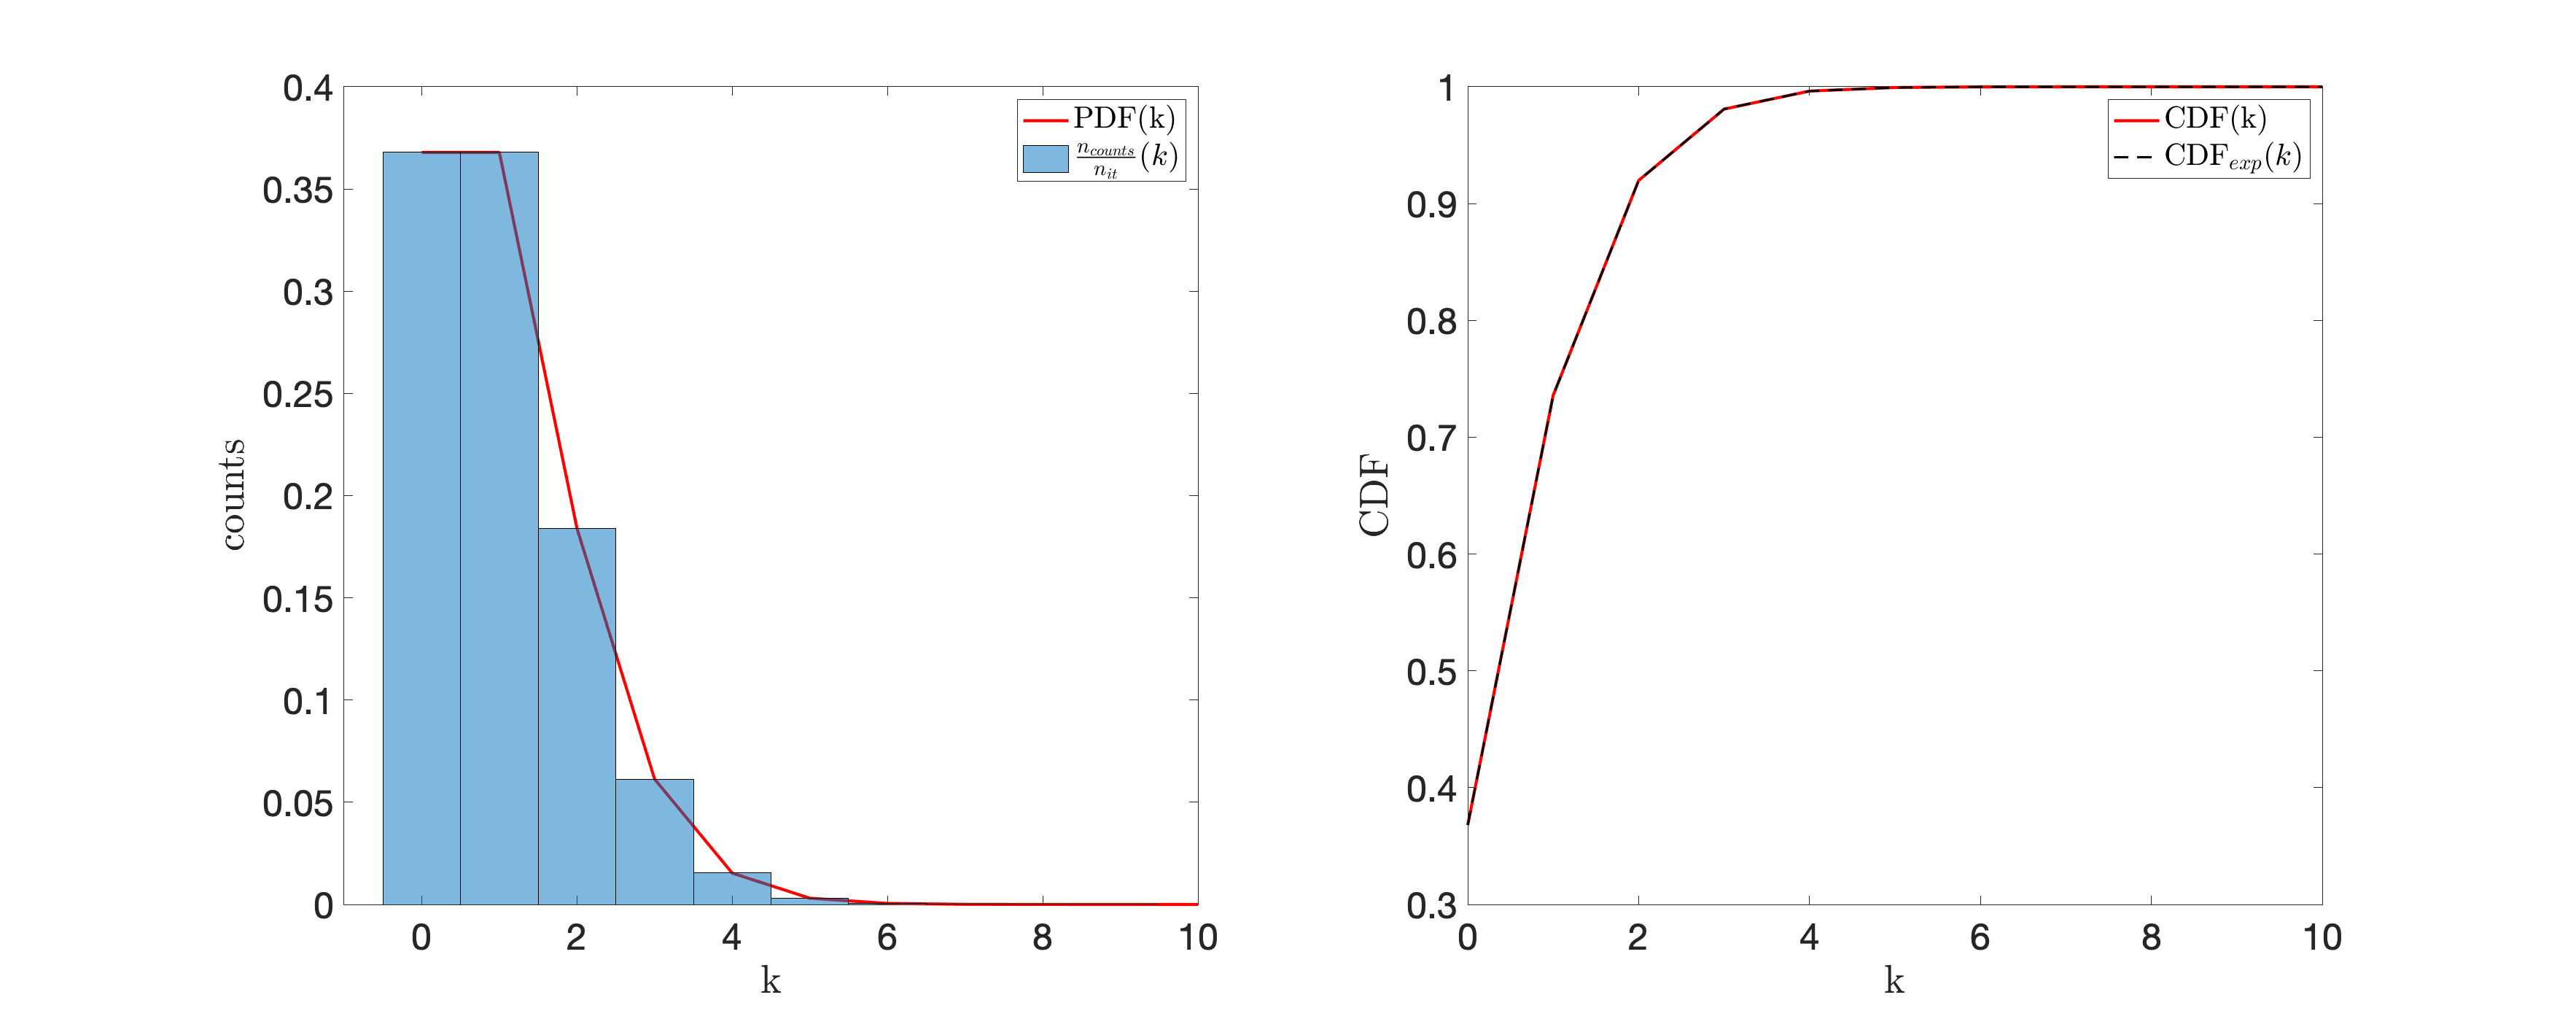
\includegraphics[width = 1 \textwidth]{Poisson_stats.eps}
	\caption{\label{Poisson_stat} Left: Normalised histogram for the number of counts obtained for each $k$ following the Poisson law of parameter $\lambda = 1$ with the expected $P(k)$ (red) - Right: $C_{exp}(k)$ obtained by summing the contributions from each bin of the histogram and $C(k)$ the theoretical cumulative distribution function for $\lambda = 1$. }
\end{figure}  

One more thing that had to be treated is the energy distribution of the emitted electrons. Indeed, all the electrons are not generated with zero velocity. The emission direction can also vary, but this will not be implemented.  Regarding the energy distribution, according to \cite{HasselII, Pagonakis}, it seems that the emitted electrons' energy follows a gamma law, such that it averages at $2$ eV. Recall that the gamma distribution varies in shape and in peak localisation according two parameters $\kappa$ and $\theta$, with $\kappa$ the shape parameter and $\theta$ the scale parameter. Recall too that the mean is given by $m=\kappa \theta$. \\

\begin{figure}[h!]
\centering
	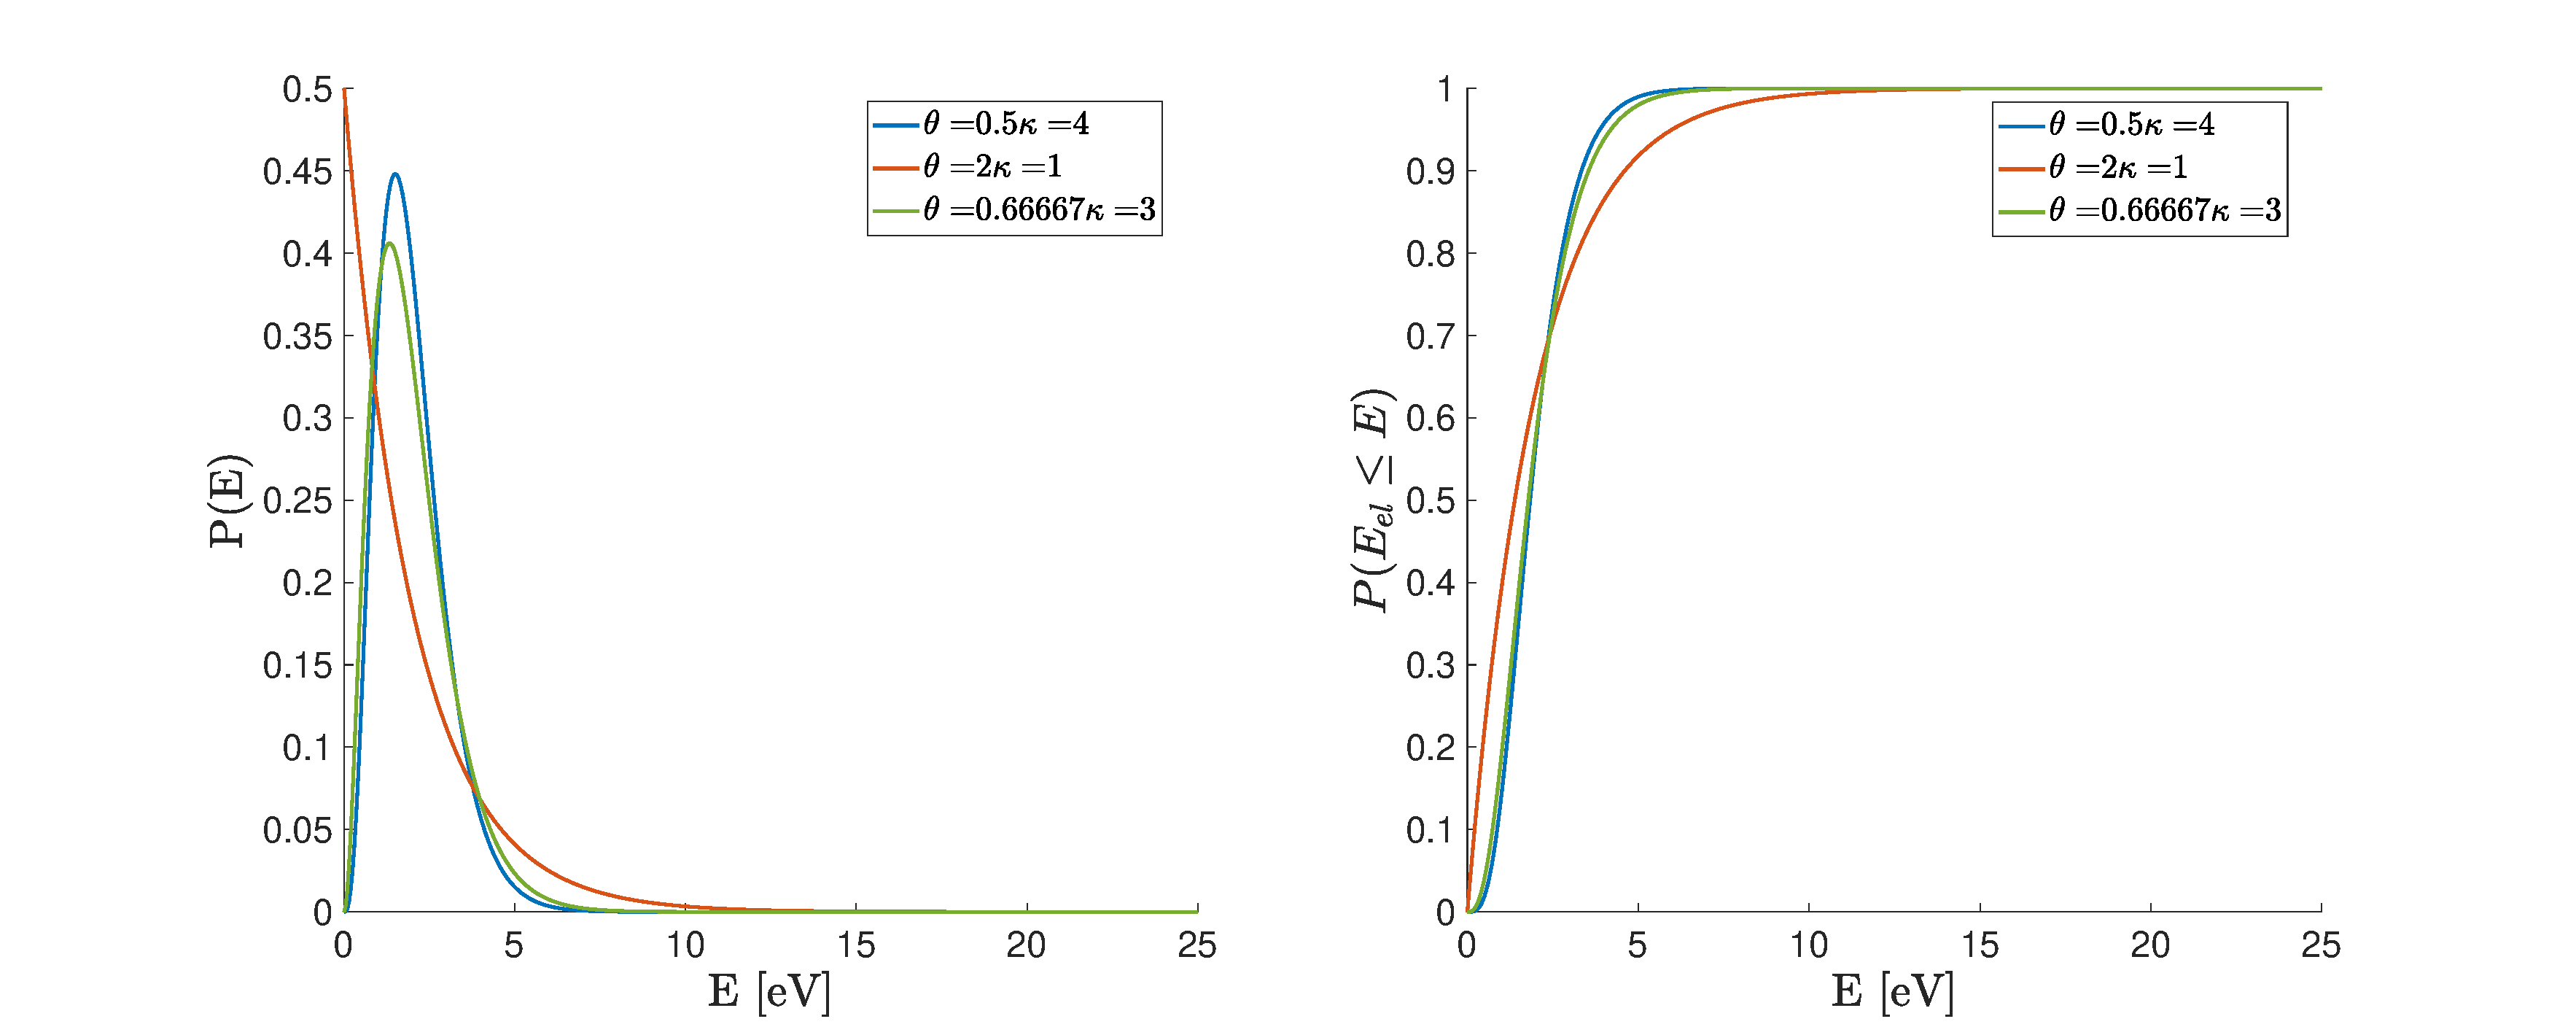
\includegraphics[width = 1 \textwidth]{Gamma_distr.eps}
	\caption{\label{Gamma_distr} Left: Gamma PDF for several $(\kappa, \theta)$ couples - Right: Corresponding CDF. }
\end{figure}  

\noindent Fig.(\ref{Gamma_distr}) shows several gamma distributions with different couples $(\kappa, \theta)$ such that $m=2$ eV. The couple that has been kept is $(\kappa,\theta) = (0.5,4)$, so the peak probability would be closer to 2 eV. Recall that the probability density function and the cumulative distribution for a gamma distribution have the following forms: 

\beq
P(E) = \frac{1}{\Gamma(\kappa)\theta^{\kappa}}E^{\kappa-1}e^{-\frac{E}{\theta}},
\eeq

\beq
C(E) = \frac{1}{\Gamma(\kappa)}\gamma{\Big(\kappa, \frac{E}{\theta}\Big)},
\eeq

\noindent where $\gamma{\Big(\kappa, \frac{E}{\theta}\Big)}$ is the lower incomplete gamma function.\\ 


\noindent Regarding the numerical implementation of the electron energy distribution in the FENNECS code, the same procedure as to produce a random number of electrons was applied, but in that case, the random numbers generated would not be integer anymore, and would follow a gamma distribution instead of Poisson. The difference in the number generation lies mostly in the discretisation of the range of values that could be taken. For Poisson generated numbers, only integer values can be taken, and hence, the construction conducted previously led to exactly Poisson distributed values. In the case of the electrons' energy, the latter can physically vary on a continuum. Our energy-values generator is hence limited by the degree of precision in the discretisation of the energy range. However, for our purpose, that is of a qualitative survey of the influence of ion-induced electrons, such precision is not required, since according to the large electric field values, no significant effect of the initial electrons' energy is to be expected. The random generation steps are listed below.

\begin{enumerate}[i)]
\item{Generate a random number $r$ uniformly  in $[0,1[. $}
\item{Evaluate the CDF of the law with  $(\kappa,\theta) = (0.5,4)$ in the range $[0,15]$ eV with $N=500$ points.}
\item{Take $E$ as $E := \min_{\tilde{E}} |r-C(\tilde{E})|$}.
\end{enumerate}

\noindent Fig.(\ref{gamma_hist}) shows that our gamma random-number generator functions correctly. Indeed, following the same procedure as to statistically test the Poisson generator, one sees that over a large number of counts, the obtained distribution matches the gamma PDF. 

\begin{figure}[h!]
\centering
	\includegraphics[width = 1 \textwidth]{gamma_hist_restr.eps}
	\caption{\label{gamma_hist} Statistical results obtained from our gamma random-number generator. The red curve represents the analytical probability density function for this particular gamma distribution. }
\end{figure}  



To put the module functioning in a nutshell, the process of generating electrons out of the ions loss consisted simply in combining the previous steps each time an ion was to hit the cathode. The full numerical treatment consisted in identifying the ions that would hit the cathode and apply the external module taking account for electron emissions. Summing up the steps, each ion that disappeared would be identified evaluating the geometric weight \cite{fennecs}, which would state that the particle is no longer in the simulation domain. Then, its energy would be evaluated, so that the average yield $\gamma(E)$ would serve in generating a random number of electrons, for which some additional memory would have been allocated. These electrons would then be placed initially at the last position \emph{inside} the domain, and be given an energy randomly generated according to the gamma law from above. The ion could then safely be removed from the particles, and the electrons would contribute to the newly updated population of particles. In light of that, it is important that the time step is short enough so the last recorded ion positions before they get removed, are close enough to the electrode, to avoid any spread effect as in Fig.(\ref{vert_spread}). However, since the electrons are to be tracked to evaluate their potential contribution to any electron cloud, the time step should be already little enough. Fig.(\ref{scheme}) illustrates the numerical treatment of cathode colliding ions. 

\begin{figure}[h!]
\centering
	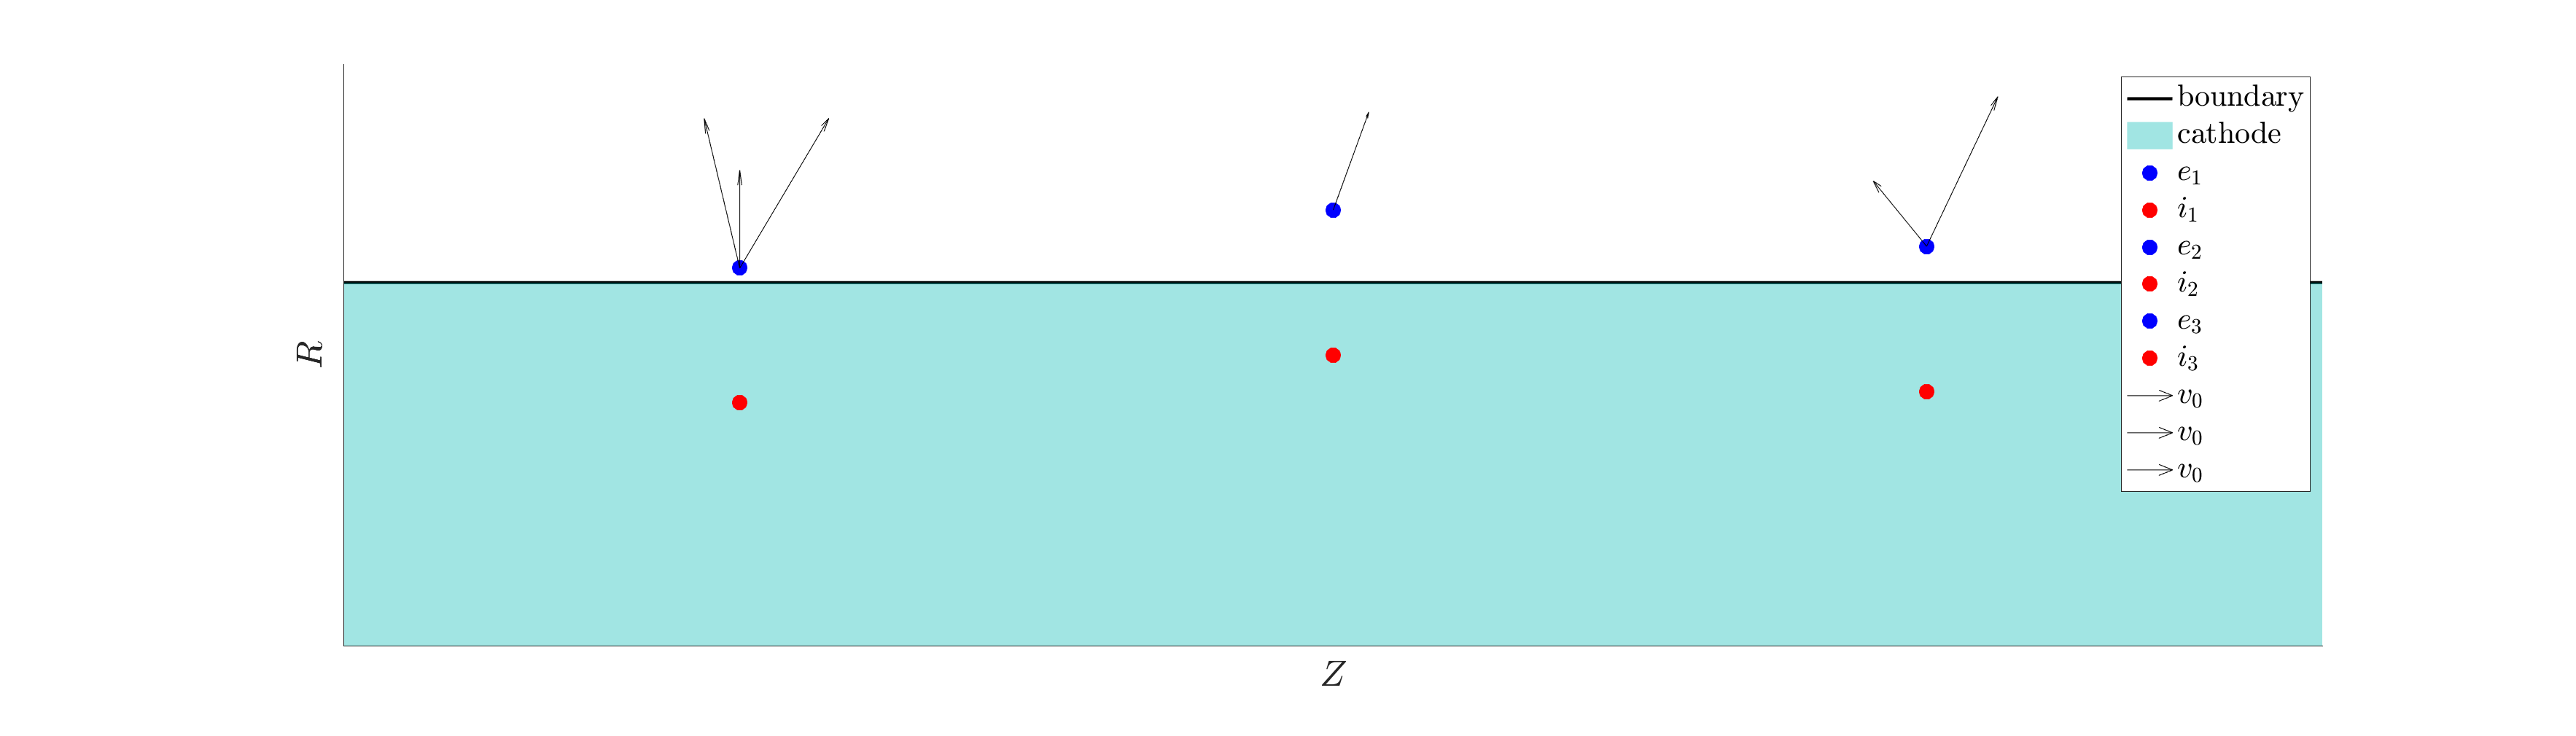
\includegraphics[width = 1 \textwidth]{electrode.eps}
	\caption{\label{scheme} Schematics of the situation where several ions are collected at the cathode, and a group of electrons is produced each time. Note that the number of electrons per incident ion is different, and the initial velocity vectors have different lengths due to the initial energy distribution}
\end{figure}  




